\begin{center}
 \textsc{Физбой, 11 класс. Полуфинал.}
\end{center}
\vspace{0.01cm}
\hrule
\parindent=0mm

\task{Найдите частоту малых колебаний математического маятника
   относительно его нижнего положения равновесия, если непосредственно
   под равновесным положением шарика на расстоянии $h$ от него
   закреплен заряд $Q$. Длина нити $l$, масса шарика $m$, заряд $q$.}

\task{Легкая нерастяжимая нить длиной $2 \unit{м}$ удерживается за
   ее концы так, что они находятся на данной высоте рядом друг с
   другом. На нити висит проволочная скобка в виде перевернутой буквы
   U. Масса скобки равна 1 грамму. Нить выдерживает максимальную
   растягивающую силу $F = 5 \unit{Н}$ ($F \gg mg$). Концы нити
   начинают перемещать в противоположных горизонтальных направлениях с
   одинаковыми скоростями $1 \mathrm{м/с}$. В какой-то момент нить не
   выдерживает и рвется. На какую максимальную высоту в момент разрыва
   нити взлетит скобка? Сопротивлением воздуха пренебречь.}

\taskpic{Над одним молем идеального газа совершают процесс, показанный на
   рисунке. Найти максимальную температуру газа в течение этого
   процесса (процесс считать квазистатическим)}{
\begin{tikzpicture}
  \draw[help lines,step=0.3] (0,0) grid (3,2.7);  
  \draw[->,thick] (0,0) -- (0,3) node[right] {\tiny{$p,\unit{кПа}$}};
  \draw[->,thick] (0,0) -- (3.5,0);
  \draw[very thick,red] (0.6,1) to[out=90,in=180] (1.2,2) to
  [out=0,in=90] (2.5,1);
  \draw (0,-0.3) node {\tiny{$0$}};
  \draw (3,0.1) -- ++(0,-0.2) node[below] {\tiny{3}};
  \draw(0.1,1.2) -- ++(-0.2,0) node[left=-3] {\tiny{2}};
  \draw(0.1,2.4) -- ++(-0.2,0) node[left=-3] {\tiny{3}};
  \draw (1.5,-0.2) node {\tiny{$V,\unit{м}^3$}};
\end{tikzpicture}
}

\taskpic{C одним молем идеального одноатомного газа провели замкнутый
цикл, изображённый на рисунке, где $1–2$ изотерма, $2–3$ изобара,
$3–4$ политропа, для которой $C = R/2$, и $4–1$ изохора. Минимальная
температура, достигаемая газом в цикле, $T_{min} = 300 \,
К$. Политропическим процессом называется процесс, происходящий с
постоянной теплоёмкостью $C$. Определите КПД цикла
$\eta$.}{
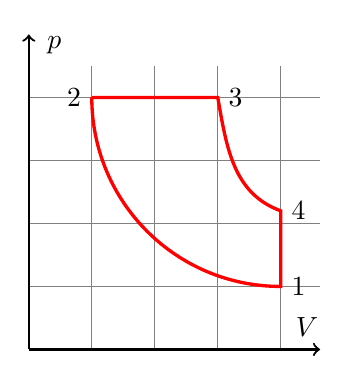
\begin{tikzpicture}
  \draw[help lines,step=0.8] (0,0) grid (3.7,3.6);  
  \draw[thick,->] (0,0) -- (3.7,0) node [above=8,left=-3] {$V$};
  \draw[thick,->] (0,0) -- (0,4) node[above=-4,right=3] {$p$};
  \draw[very thick,red] (0.8,3.2) node[black,left] {2} -- (2.4,3.2)
  node[black,right] {3} to[out=-80,in=160]
  (3.2,0.8*2.2) node[black,right] {4} -- (3.2,0.8) node[black,right] {1} to [out=180,in=-90]
  (0.8,3.2);
\end{tikzpicture}
}

\task{В схеме, изображенной на рисунке, имеются четыре диода. Известно, что при любом
   напряжении, подведенном к выводам схемы, ток через амперметр не течет. ВАХ трех диодов $D1$, $D2$ и
   $D3$ известны (см. график). Постройте ВАХ четвертого диода.
}

\begin{center}
  \parbox{4.5cm}{\begin{circuitikz}
  \draw[o-,thick](0,1) -- (0.5,1) -- (0.5,2);
  \draw[thick] (0.5,2) to[Do,l=$D_1$] (2,2) to [Do,l=$D_2$] (3.5,2) -- (3.5,1);
  \draw[thick,-o] (3.5,1) -- (4,1);
  \draw[thick] (0.5,1) -- (0.5,0) to[Do,l_=$D_3$] (2,0) to[Do,l_=$D_4$] (3.5,0) -- (3.5,1);
  \draw[thick] (2,2) to[ammeter] (2,0);
\end{circuitikz}}%
\parbox{4.5cm}{\begin{tikzpicture}[scale=1.2]
  \draw[help lines,step=0.5] (0,0) grid (2.5,2);  
  \draw[thick,->] (0,0) -- (2.7,0) node[above] {\tiny{$U,\unit{В}$}};
  \draw[thick,->] (0,0) -- (0,2.5) node[left] {\tiny{$I,\unit{A}$}};
  \draw[red,thick,domain=0:0.75] plot(\x,5*\x*\x*\x) node[above] {\tiny{$D_1$}};
  \draw[green,thick,domain=0:1.62] plot(\x,0.5*\x*\x*\x) node[above] {\tiny{$D_2$}};
  \draw[blue,thick,domain=0:2.2] plot(\x,0.2*\x*\x*\x) node[above]
  {\tiny{$D_3$}};
  \foreach \x in {1,2,3,4,5} \draw (\x/2,0.1) -- +(0,-0.2)
  node[below=-2] {\tiny{\x}};
  \foreach \y in {0.1,0.2,0.3,0.4} \draw (0.1,5*\y) -- +(-0.2,0) node[left=-2] {\tiny{\y}};
\end{tikzpicture}
}
\end{center}


\taskpic{В архиве Снеллиуса найден чертеж оптической схемы. От времени
  чернила выцвели и на чертеже остались видны только три точки ---
  фокус линзы $F$, источник света $S$, точка $L$, принадлежащая
  плоскости тонкой линзы, и часть прямой линии а, соединяющий источник
  света и его изображение $S'$. Из пояснений к чертежу следует, что
  точка $S'$ отстоит от плоскости линзы на расстояние, большим, чем
  точка $S$.  Возможно ли по этим данным восстановить исходную схему?
  Если да, то покажите, как это сделать. Чему равно фокусное
  расстояние линзы?  }{
\begin{tikzpicture}
  \draw[very thick] (0.5,3.5) -- ++(1.5,-1);
  \draw[very thick,dashed] (2,2.5) -- +(1,-2/3);
  \draw[thick] (2.4,1.5) node[left] {$F$}  -- (2.6,1.5);
  \draw[thick] (2.5,1.6)  -- (2.5,1.4);
  \draw[thick] (3.4,1) node[below] {$L$}  -- (3.6,1);
  \draw[thick] (3.5,1.1)  -- (3.5,0.9);
  \draw[fill=black] ($(0.5,3.5)!0.15!(2,2.5)$) circle (0.05)
  node[above] {$S$};
  \draw[fill=black] (2,2.5) circle (0.05) node[above] {$a$};
\end{tikzpicture}
}

\setcounter{notask}{1}